%%%%%%%%%%%%%%%%%%%%%%%%%%%%%%%%%%%%%%%%%
% University/School Laboratory Report
% LaTeX Template
% Version 3.1 (25/3/14)
%
% This template has been downloaded from:
% http://www.LaTeXTemplates.com
%
% Original author:
% Linux and Unix Users Group at Virginia Tech Wiki 
% (https://vtluug.org/wiki/Example_LaTeX_chem_lab_report)
%
% License:
% CC BY-NC-SA 3.0 (http://creativecommons.org/licenses/by-nc-sa/3.0/)
%
%%%%%%%%%%%%%%%%%%%%%%%%%%%%%%%%%%%%%%%%%

%----------------------------------------------------------------------------------------
%	PACKAGES AND DOCUMENT CONFIGURATIONS
%----------------------------------------------------------------------------------------

\documentclass{article}

\usepackage[version=3]{mhchem} % Package for chemical equation typesetting
\usepackage{siunitx} % Provides the \SI{}{} and \si{} command for typesetting SI units
\usepackage{graphicx} % Required for the inclusion of images
\usepackage{natbib} % Required to change bibliography style to APA
\usepackage{amsmath} % Required for some math elements 
\usepackage{gensymb}
\usepackage{textcomp}

\setlength\parindent{0pt} % Removes all indentation from paragraphs

\renewcommand{\labelenumi}{\alph{enumi}.} % Make numbering in the enumerate environment by letter rather than number (e.g. section 6)

%\usepackage{times} % Uncomment to use the Times New Roman font

%----------------------------------------------------------------------------------------
%	DOCUMENT INFORMATION
%----------------------------------------------------------------------------------------

\title{ECSE 426 \\ Analog Data Acquisition, Digitizing\\ Filtering, and Digital I/O} % Title

\begin{document}

\maketitle % Insert the title, author and date

\begin{center}
\begin{tabular}{l r}
Date Performed: & Feb 17, 2017 \\ % Date the experiment was performed
Students: & Jaeho Lee (260633759) \\ % Partner names
& Bobak Baghi \\
Instructor: & Professor Zeljko Zilic % Instructor/supervisor
\end{tabular}
\end{center}

\date{\today} % Date for the report

% If you wish to include an abstract, uncomment the lines below
% \begin{abstract}
% Abstract text
% \end{abstract}

%----------------------------------------------------------------------------------------
%	SECTION 1
%----------------------------------------------------------------------------------------

\section{Abstract}

Micro-Controllers commonly have multiple different sensors to receive analogue data. Temperature sensor is one of the critical sensors which checks whether microchip is not overheating which can damage chip. This experiment is mainly focusing on receiving temperature of microchip using temperature sensor. Additionally, a LED display was used to display the temperature data. The system was designed to display temperature in Celsius.  When an user interface (switch) receives signal, the temperature in Fahrenheit would display. A FIR filter was implemented to filter out noisy data read from the sensor.

%----------------------------------------------------------------------------------------
%	SECTION 2
%----------------------------------------------------------------------------------------

\section{Problem Statement}

%----------------------------------------------------------------------------------------
%	SECTION 3
%----------------------------------------------------------------------------------------

\section{Theory and Hypothesis}
\subsection{Temperature Calculation}
The analogue data of sensor is in voltage. Analogue to Digital Converter (ADC) in this experiment uses 12 bit data which gives 4096 different inputs. The sensor can measure temperature between \(-40\, \celsius ~ 125\, \celsius \). Equation (1) was used to calculate temperature in Celsius. Equation (2) was used to convert Celsius data into Fahrenheit.\\
\begin{equation}
temperature(\, \celsius) = 400*S*\frac{3.6}{4096} + 25
\end{equation}\\
\begin{equation}
temperature(^{\circ}F) = 1.8*temperature(\, \celsius) + 32
\end{equation}\\
\subsection{Data Display}
For displaying data, four digit 7-segment display was used. Individual segment can be controlled by using general purpose input output (GPIO) pins implemented on the Micro-controller unit. Figure 1 shows how 7-segment LCD display is consisted.

\begin{figure}[h]
\begin{center}
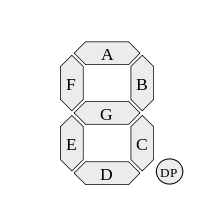
\includegraphics[width=0.50\textwidth]{7segment} % Include the image placeholder.png
\caption{7-segment LED display}
\end{center}
\end{figure}
To display each digit from 0 to 9, each number was defined separately. List of bit sequence to display number is follow in table.
\begin{center}
\begin{tabular}{lclclclclclc|cl}
a&b&c&d&e&f&g&display\\
\hline
1&1&1&1&1&1&0&0\\
0&1&1&0&0&0&0&1\\
1&1&0&1&1&0&1&2\\
1&1&1&1&0&0&1&3\\
0&1&1&0&0&1&1&4\\
1&0&1&1&0&1&1&5\\
0&0&1&1&1&1&1&6\\
1&1&1&0&0&0&0&7\\
1&1&1&1&1&1&1&8\\
1&1&1&0&0&1&1&9
\end{tabular}
\end{center}

\subsection{Data Filtering}
FIR filter was used 


%----------------------------------------------------------------------------------------
%	SECTION 4
%----------------------------------------------------------------------------------------

\section{Implementation}

The atomic weight of magnesium is concluded to be \SI{24}{\gram\per\mol}, as determined by the stoichiometry of its chemical combination with oxygen. This result is in agreement with the accepted value.

\begin{figure}[h]
\begin{center}

\includegraphics[width=0.65\textwidth]{placeholder} % Include the image placeholder.png
\caption{Figure caption.}
\end{center}
\end{figure}

%----------------------------------------------------------------------------------------
%	SECTION 5
%----------------------------------------------------------------------------------------

\section{Observation}

The accepted value (periodic table) is \SI{24.3}{\gram\per\mole} \cite{Smith:2012qr}. The percentage discrepancy between the accepted value and the result obtained here is 1.3\%. Because only a single measurement was made, it is not possible to calculate an estimated standard deviation.

The most obvious source of experimental uncertainty is the limited precision of the balance. Other potential sources of experimental uncertainty are: the reaction might not be complete; if not enough time was allowed for total oxidation, less than complete oxidation of the magnesium might have, in part, reacted with nitrogen in the air (incorrect reaction); the magnesium oxide might have absorbed water from the air, and thus weigh ``too much." Because the result obtained is close to the accepted value it is possible that some of these experimental uncertainties have fortuitously cancelled one another.

%----------------------------------------------------------------------------------------
%	SECTION 6
%----------------------------------------------------------------------------------------

\section{Conclusion}

\begin{enumerate}
\begin{item}
The \emph{atomic weight of an element} is the relative weight of one of its atoms compared to C-12 with a weight of 12.0000000$\ldots$, hydrogen with a weight of 1.008, to oxygen with a weight of 16.00. Atomic weight is also the average weight of all the atoms of that element as they occur in nature.
\end{item}
\begin{item}
The \emph{units of atomic weight} are two-fold, with an identical numerical value. They are g/mole of atoms (or just g/mol) or amu/atom.
\end{item}
\begin{item}
\emph{Percentage discrepancy} between an accepted (literature) value and an experimental value is
\begin{equation*}
\frac{\mathrm{experimental\;result} - \mathrm{accepted\;result}}{\mathrm{accepted\;result}}
\end{equation*}
\end{item}
\end{enumerate}

%----------------------------------------------------------------------------------------
%	BIBLIOGRAPHY
%----------------------------------------------------------------------------------------

\bibliographystyle{apalike}

\bibliography{sample}

%----------------------------------------------------------------------------------------


\end{document}